% This is a Basic Assignment Paper but with like Code and stuff allowed in it. 

\documentclass[11pt]{article}

% Preamble

\usepackage[margin=1in]{geometry}
\usepackage{amsfonts, amsmath, amssymb}
\usepackage{fancyhdr, float, graphicx}
\usepackage[utf8]{inputenc} % Required for inputting international characters
\usepackage[T1]{fontenc} % Output font encoding for international characters
\usepackage{fouriernc} % Use the New Century Schoolbook font
\usepackage[nottoc, notlot, notlof]{tocbibind}
\usepackage{listings}
\usepackage{xcolor}

\definecolor{codegreen}{rgb}{0,0.6,0}
\definecolor{codegray}{rgb}{0.5,0.5,0.5}
\definecolor{codepurple}{rgb}{0.58,0,0.82}
\definecolor{backcolour}{rgb}{0.95,0.95,0.92}

\lstdefinestyle{mystyle}{
    backgroundcolor=\color{backcolour},   
    commentstyle=\color{codegreen},
    keywordstyle=\color{magenta},
    numberstyle=\tiny\color{codegray},
    stringstyle=\color{codepurple},
    basicstyle=\ttfamily\footnotesize,
    breakatwhitespace=false,         
    breaklines=true,                 
    captionpos=b,                    
    keepspaces=true,                 
    numbers=left,                    
    numbersep=5pt,                  
    showspaces=false,                
    showstringspaces=false,
    showtabs=false,                  
    tabsize=2
}

\lstset{style=mystyle}

% Header and Footer
\pagestyle{fancy}
\fancyhead{}
\fancyfoot{}
\fancyhead[L]{\textit{\Large{OOPJC Assignment 8protected
protected
protected}}}
%\fancyhead[R]{\textit{something}}
\fancyfoot[C]{\thepage}
\renewcommand{\footrulewidth}{1pt}



% Other Doc Editing
% \parindent 0ex
%\renewcommand{\baselinestretch}{1.5}

\begin{document}

\begin{titlepage}
	\centering

	%---------------------------NAMES-------------------------------

	\huge\textsc{
		MIT World Peace University
	}\\

	\vspace{0.75\baselineskip} % space after Uni Name

	\LARGE{
		Object Oriented Programming with Java and C++\\
		Second Year B. Tech, Semester 1
	}

	\vfill % space after Sub Name

	%--------------------------TITLE-------------------------------

	\rule{\textwidth}{1.6pt}\vspace*{-\baselineskip}\vspace*{2pt}
	\rule{\textwidth}{0.6pt}
	\vspace{0.75\baselineskip} % Whitespace above the title



	\huge{\textsc{
			Developing a Simple Graphical Calculator using Swing in Java
		}} \\



	\vspace{0.5\baselineskip} % Whitespace below the title
	\rule{\textwidth}{0.6pt}\vspace*{-\baselineskip}\vspace*{2.8pt}
	\rule{\textwidth}{1.6pt}

	\vspace{1\baselineskip} % Whitespace after the title block

	%--------------------------SUBTITLE --------------------------	

	\LARGE\textsc{
		Practical Report\\
		Assignment 8
	} % Subtitle or further description
	\vfill

	%--------------------------AUTHOR-------------------------------

	Prepared By
	\vspace{0.5\baselineskip} % Whitespace before the editors

	\Large{
		Krishnaraj Thadesar \\
		Cyber Security and Forensics\\
		Batch A1, PA 20
	}


	\vspace{0.5\baselineskip} % Whitespace below the editor list
	\today

\end{titlepage}


\tableofcontents
\thispagestyle{empty}
\clearpage


\setcounter{page}{1}

\section{Aim and Objectives}
\subsection*{Aim}
To Develop a simple calculator using Swing in Java
\subsection*{Objective}
\begin{enumerate}
	\item To understand concept of AWT and Java swings
	\item To explore Java Swing containers
\end{enumerate}
\section{Problem Statement}
Write a Java program to create a simple calculator with the help of java swing.

\section{Theory}
\subsection{Java Swing containers}
\textit{Containers are an integral part of SWING GUI components. A container provides a space where a component can be located. A Container in AWT is a component itself and it provides the capability to add a component to itself. Following are certain noticable points to be considered.}

\begin{enumerate}
	\item Panel: JPanel is the simplest container. It provides space in which any other component can be placed, including other panels.

	\item Frame: A JFrame is a top-level window with a title and a border.

	\item Window: A JWindow object is a top-level window with no borders and no menubar.
\end{enumerate}
\begin{figure}[H]
	\centering
	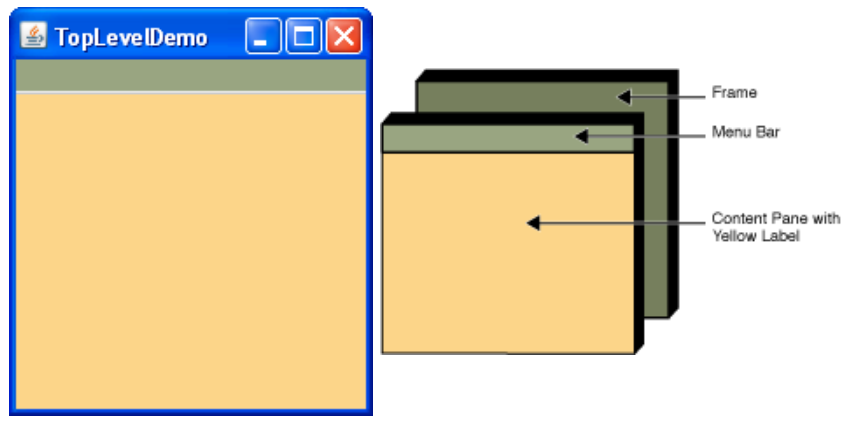
\includegraphics[scale=0.5]{containers.png}
	\caption{Top level containers in Java}
\end{figure}
\subsection{Container classes of Java Swing with examples}
\subsubsection{JPanel}
A panel is a component that is contained inside a frame window. A frame can have more than one-panel components inside it with each panel component having several other components.
\begin{lstlisting}[language=Java]
import javax.swing.*;
class JPanelExample {
    JPanelExample(){
        JFrame frame = new JFrame("Panel Example"); //create a frame
        JPanel panel = new JPanel(); //Create JPanel Object
        panel.setBounds(40,70,100,100); //set dimensions for Panel
        JButton b = new JButton("ButtonInPanel"); //create JButton object
        b.setBounds(60,50,80,40); //set dimensions for button
        panel.add(b);   //add button to the panel
        frame.add(panel);   //add panel to frame
        frame.setSize(400,400);
        frame.setLayout(null);
        frame.setVisible(true);
    }
 
}
public class Main {
    public static void main(String[] args) {
      new JPanelExample(); //create an object of FrameInherited class
    }
}
\end{lstlisting}
\subsubsection{JFrame}

A Frame, in general, is a container that can contain other components such as buttons, labels, text fields, etc. A Frame window can contain a title, a border, and also menus, text fields, buttons, and other components. An application should contain a frame so that we can add components inside it.

The Frame in Java Swing is defined in class javax.swing.JFrame. JFrame class inherits the java.awt.Frame class. JFrame is like the main window of the GUI application using swing.

\begin{lstlisting}[language=Java]
import javax.swing.*;
class FrameInherited extends JFrame{    //inherit from JFrame class
    JFrame f;
    FrameInherited(){
        JButton b=new JButton("JFrame_Button");//create button object
        b.setBounds(100,50,150, 40);
 
        add(b);//add button on frame
        setSize(300,200);
        setLayout(null);
        setVisible(true);
    }
}
public class Main {
    public static void main(String[] args) {
      new FrameInherited(); //create an object of FrameInherited class
    }
}
\end{lstlisting}
\subsubsection{JWindow}
The class JWindow is a container that can be displayed but does not have the title bar or window-management buttons.
\begin{lstlisting}[language=Java]
import java.awt.*;
import java.awt.event.*;
import javax.swing.*;

class SwingContainerDemo {
    private JFrame mainFrame;
    private JLabel headerLabel;
    private JLabel statusLabel;
    private JPanel controlPanel;
    private JLabel msglabel;

    public SwingContainerDemo() {
        prepareGUI();
    }

    public static void main(String[] args) {
        SwingContainerDemo swingContainerDemo = new SwingContainerDemo();
        swingContainerDemo.showJWindowDemo();
    }

    private void prepareGUI() {
        mainFrame = new JFrame("Java Swing Examples");
        mainFrame.setSize(400, 400);
        mainFrame.setLayout(new GridLayout(3, 1));

        mainFrame.addWindowListener(new WindowAdapter() {
            public void windowClosing(WindowEvent windowEvent) {
                System.exit(0);
            }
        });
        headerLabel = new JLabel("", JLabel.CENTER);
        statusLabel = new JLabel("", JLabel.CENTER);
        statusLabel.setSize(350, 100);

        controlPanel = new JPanel();
        controlPanel.setLayout(new FlowLayout());

        mainFrame.add(headerLabel);
        mainFrame.add(controlPanel);
        mainFrame.add(statusLabel);
        mainFrame.setVisible(true);
    }
    private void showJWindowDemo() {
        headerLabel.setText("Container in action: JWindow");
        mainFrame.setVisible(true);
    }

}
\end{lstlisting}
\subsection{Swing components including buttons, checkboxes, sliders, and list boxes, etc.}
There are many imporant Swing components that allow us to design GUIs. Here are some of them.
\begin{itemize}
	\item \textbf{JTextArea}: TextArea defines an editable text field. It can have multiple lines. The swing class that defines the text area is JTextArea and it inherits the JTextComponent class.
	\item \textbf{JButton}: A button is a component that is used to create a push button with a name or label on it. In swing, the class that creates a labeled button is JButton. JButton inherits the AbstractButton class. We can associate the ActionListener event to the button to make it take some action when it is pushed.
	\item \textbf{JList}: A list consists of multiple text items. Users can either select a single item \textbf{or} multiple items at a time. The class that implements the list in swing API is JList. JList is a descendent of the JComponent class.
	\item \textbf{JComboBox}: The JCombobox class shows a list of choices from which a user can select an option. The selected choice is at the top. JComboBox derives from the JComponent class.
	\item \textbf{JSlider}: A slider allows us to select a specific range of values. In Java Swing API, JSlider is the class that is used to implement the slider.
	\item \textbf{JCheckBox}: The JcheckBox class is used to create chekbox in swing framework.
	\item \textbf{JRadioButton}: Radio button is a group of related button in which only one can be selected. JRadioButton class is used to create a radio button in Frames.
	\item \textbf{JLabel}: In Java, Swingtoolkit contains a JLabel Class. It is under package javax.swing.JLabel class. It is used for placing text in a box. Only Single line text is allowed and the text can not be changed directly.
	\item \textbf{JPasswordField}: In Java, Swing toolkit contains a JPasswordField Class. It is under package javax.swing.JPasswordField class. It is specifically used for password and it can be edited.
\end{itemize}
\subsection{Heavyweight Components and Lightweight Components}
There are two kinds of graphics components in the Java programming language: heavyweight and lightweight.\\

\textit{A component is said to be a heavyweight component if it uses native code provided by your computer's operating system to display buttons, choice lists, text fields, and the like. Such operating-system routines are said to be the components's peers.}\\

\textit{A Swing component is said to be a lightweight component because it written entirely in Java and does the high-level display work itself, rather than relying on code provided by your computer's operating system.}

\subsection{What is Double Buffering?}
\begin{enumerate}
	\item Double-buffering is the process of drawing graphics into an off-screen image buffer and then copying the contents of the buffer to the screen all at once.
	\item For the complex graphics, using double-buffering can reduce flickering issues.
	\item Java Swing automatically supports double-buffering for all of its components.
	\item Double-buffering is memory intensive, its use is only justified for components that are repainted very frequently or have particularly complex graphics to display.
	\item If a container uses double-buffering, any double-buffered children it has shared the off-screen buffer of the container, the required off-screen buffer is never larger than the on-screen size of the application.
	\item To enable double buffering, simply call the setDoubleBuffered() method (inherited from JComponent) to set the double-buffered property to true for any components that should use double-buffered drawing.
\end{enumerate}
\subsection{Difference between applet and Swing}
Applet is a Java program that can be embedded into a web page. It runs inside the web browser and works at client side. An applet is embedded in an HTML page using the APPLET or OBJECT tag and hosted on a web server.
They are used to make the web site more dynamic and entertaining. All applets are sub-classes (either directly or indirectly) of java.applet.Applet class. Applets are not stand-alone programs. Instead, they run within either a web browser or an applet viewer. JDK provides a standard applet viewer tool called applet viewer. \\

Swing in Java is a lightweight GUI toolkit which has a wide variety of widgets for building optimized window based applications. It is a part of the JFC( Java Foundation Classes). It is build on top of the AWT API and entirely written in java.\\

It is platform independent unlike AWT and has lightweight components. It becomes easier to build applications since we already have GUI components like button, checkbox etc. This is helpful because we do not have to start from the scratch.

\section{Platform}
\textbf{Operating System}: Arch Linux x86-64 \\
\textbf{IDEs or Text Editors Used}: Visual Studio Code\\
\textbf{Compilers} : g++ and gcc on linux for C++, and javac, with JDK 18.0.2 for Java\\

\section{Input}
The numbers and the Operators.

\section{Output}
The Output of the entered Calculation in the Display Section of the Calculator
\begin{figure}[H]
	\centering
	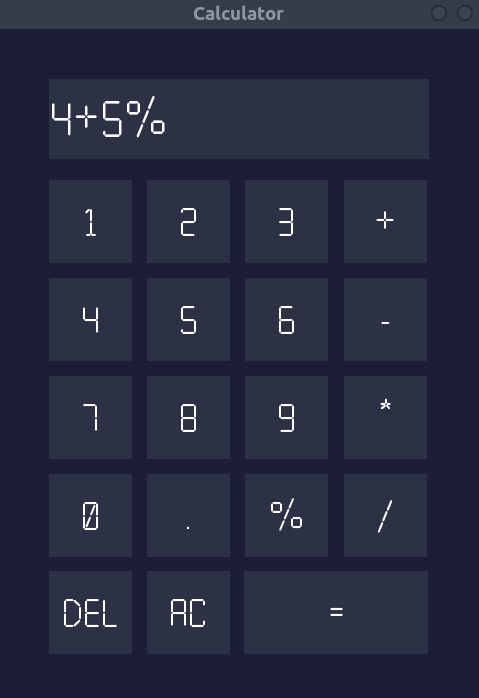
\includegraphics[scale=0.5]{Calculator.png}
	\caption{Calculator with Java Swing}
\end{figure}

\section{Code}

\lstinputlisting[language=java, caption=Calculator.java]{../Programs/java_implementations/assignment_8/Calculator/src/main/java/org/OOPCJ/Krishnaraj/Main.java}

\section{Dependencies}
\lstinputlisting[language=java, caption=pom.xml]{../Programs/java_implementations/assignment_8/Calculator/pom.xml}

\section{Conclusion}
Thus, implemented simple calculator with the help of java swing and performed various
operations.

% \pagebreak

\section{FAQs}
\begin{enumerate}
	\item \textit{Methods of component class in Java Swing?}\\

	      A component is an object having a graphical representation that can be displayed on the screen and that can interact with the user. Examples of components are the buttons, checkboxes, and scrollbars of a typical graphical user interface.\\

	      The Component class is the abstract superclass of the nonmenu-related Abstract Window Toolkit components. Class Component can also be extended directly to create a lightweight component. A lightweight component is a component that is not associated with a native window. On the contrary, a heavyweight component is associated with a native window. The isLightweight() method may be used to distinguish between the two kinds of the components.

	      Some methods of this class are:
	      \begin{itemize}
		      \item \textbf{void add(PopupMenu):} Adds the specified popup menu to the component.
		      \item \textbf{void addComponentListener(ComponentListener):} Adds the specified component listener to receive component events from this component.
		      \item \textbf{void addFocusListener(FocusListener):} Adds the specified focus listener to receive focus events from this component when this component gains input focus.
		      \item \textbf{Rectangle getBounds(): Gets} the bounds of this component in the form of a Rectangle object.
		      \item \textbf{Rectangle getBounds(Rectangle):} Stores the bounds of this component into "return value" rv and return rv.
	      \end{itemize}

	\item \textit{Ways to create a frame in Java Swing? Explain with examples}
	      \begin{enumerate}
		      \item By creating the object of Frame class (association)
		            \begin{lstlisting}[language=Java]
// Java program to create frames
// using association

import javax.swing.*;
public class test1
{
	JFrame frame;

	test1()
	{
		// creating instance of JFrame with name "first way"
		frame=new JFrame("first way");
		
		// creates instance of JButton
		JButton button = new JButton("let's see");

		button.setBounds(200, 150, 90, 50);
		
		// setting close operation
		frame.setDefaultCloseOperation(JFrame.EXIT_ON_CLOSE);

		// adds button in JFrame
		frame.add(button);

		// sets 500 width and 600 height
		frame.setSize(500, 600);
		
		// uses no layout managers
		frame.setLayout(null);
		
		// makes the frame visible
		frame.setVisible(true);
	}
	
	public static void main(String[] args)
	{
		new test1();
	}
}

\end{lstlisting}
		      \item By extending Frame class (inheritance)
		            \begin{lstlisting}[language=Java]
// Java program to create a
// frame using inheritance().

import javax.swing.*;

// inheriting JFrame
public class test2 extends JFrame
{
	JFrame frame;
	test2()
	{
		setTitle("this is also a title");

		// create button
		JButton button = new JButton("click");

		button.setBounds(165, 135, 115, 55);
		
		// adding button on frame
		add(button);

		// setting close operation
		setDefaultCloseOperation(JFrame.EXIT_ON_CLOSE);

		setSize(400, 500);
		setLayout(null);
		setVisible(true);
	}
	
	public static void main(String[] args)
	{
		new test2();
	}
}
			
		\end{lstlisting}
		      \item Create a frame using Swing inside main()
		            \begin{lstlisting}[language=Java]
// Java program to create a frame
// using Swings in main().

import javax.swing.*;
public class Swing_example
{
	public static void main(String[] args)
	{
		// creates instance of JFrame
		JFrame frame1 = new JFrame();

		// creates instance of JButton
		JButton button1 = new JButton("click");
		JButton button2 = new JButton("again click");

		// x axis, y axis, width, height
		button1.setBounds(160, 150 ,80, 80);
		button2.setBounds(190, 190, 100, 200);

		// adds button1 in Frame1
		frame1.add(button1);
		
		// adds button2 in Frame1
		frame1.add(button2);

		// 400 width and 500 height of frame1
		frame1.setSize(400, 500) ;
		
		// uses no layout managers
		frame1.setLayout(null);
		
		// makes the frame visible
		frame1.setVisible(true);
	}
}

			  \end{lstlisting}
	      \end{enumerate}

	\item \textit{What are the Methods of JLabel class in Java Swing?}
	      \begin{itemize}
		      \item \textbf{String getText()}: Returns the text string that the label displays.
		      \item \textbf{LabelUI getUI()}: Returns the LF object that renders this component.
		      \item \textbf{String getUIClassID()}: Returns a string that specifies the name of the lf class that renders this component.
		      \item \textbf{void setIcon(Icon icon)}: Defines the icon this component will display.
		      \item \textbf{void setIconTextGap(int iconTextGap)}: If both the icon and text properties are set, this property defines the space between them.
		      \item \textbf{void setLabelFor(Component c)}: Set the component this is labelling.
		      \item \textbf{void setText(String text)}: Defines the single line of text this component will display.
		      \item \textbf{void setUI(LabelUI ui)}: Sets the LF object that renders this component.
		      \item \textbf{void setVerticalAlignment(int alignment)}: Sets the alignment of the label's contents along the Y axis.
		      \item \textbf{void setVerticalTextPosition(int textPosition)}: Sets the vertical position of the label's text, relative to its image.
		      \item \textbf{void updateUI()}: Resets the UI property to a value from the current look and feel.
	      \end{itemize}
	\item \textit{What are the Methods of AbstractButton class in Java Swing?}
	\begin{itemize}
		\item \textbf{protected ActionListener actionListener}: The button model's ActionListener.
		\item \textbf{protected ChangeEvent changeEvent}: Only one ChangeEvent is needed per button instance since the event's only state is the source property.
		\item \textbf{protected ChangeListener changeListener}: The button model's changeListener.
	\end{itemize}
	\item \textit{Write a simple Java Swing program of displaying image on the button?}
	      \begin{lstlisting}[language=Java]
import javax.swing.*;
import java.awt.event.*;
import java.awt.*;

class test extends JFrame {

    test() {
        JButton bt1 = new JButton("no"); // Creating a Yes Button.
        setDefaultCloseOperation(JFrame.EXIT_ON_CLOSE); // setting close operation.
        bt1.setBounds(60, 50, 500, 500);
        ImageIcon imageIcon = new ImageIcon("../../Lab/pic.jpg");
        bt1.setIcon(imageIcon);
        setLayout(null); // setting layout using FlowLayout object
        setSize(700, 700); // setting size of Jframe
        add(bt1); // adding Yes button to frame.
        setVisible(true);
    }

    public static void main(String[] args) {
        new test();
    }
}
\end{lstlisting}

	      \begin{figure}[H]
		      \centering
		      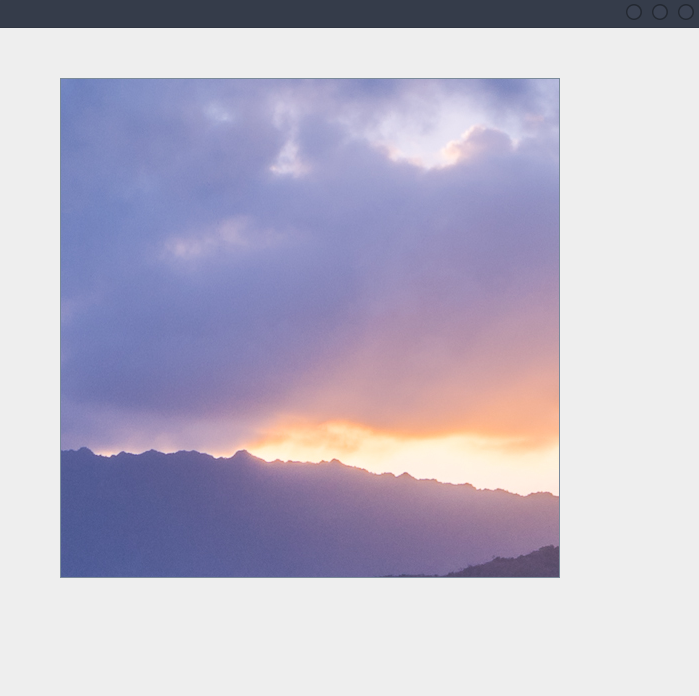
\includegraphics[scale=0.5]{buttonpic.png}
		      \caption{Button with a background image in its background. }
	      \end{figure}
\end{enumerate}

\end{document}